\chapter{Discussion}
\section{Tau}
\begin{figure}[h!tb]
\centering
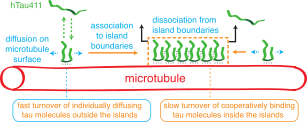
\includegraphics[scale=1]{Figures/tau8.png}
\caption[Schematic representation of island formation.]{
\textbf{Schematic representation of island formation.} Tau molecules bind and unbind with high rates to microtubules, on which they diffuse (fast turnover). When encountering an island (dashed orange box), tau molecules cooperatively associate with the island at its boundaries, rendering the tau molecules stationary, decreasing their unbinding rate (slow turnover), and causing the island to grow in size laterally. Tau molecules from solution can only bind to the inside of an island via displacement of an island-associated tau molecule, resulting in the observed concentration-dependent turnover of tau inside islands. After removal of tau from solution, tau molecules dissociate from the island boundaries, making the island shrink in size laterally.
	}\label{tau8}
\end{figure}
In our investigation of tau interactions with microtubules, we have contributed to our understanding of the distinct binding modes of tau to the microtubule. While the diffusive binding mode was already well-described, our key contribution is that tau can cooperatively bind to form cohesive islands on the microtubule. Our findings, coupled with complementary work by \cite{tan2019microtubules}, paint a detailed picture of tau's multifaceted behavior on microtubules.\par

The cooperative binding mode results in a population of stationary tau molecules characterized by remarkably low turnover rates. This is in contrast to the diffusive mode, where tau molecules exhibit high turnover rates. At physiological concentrations, these two distinct populations coexist on the microtubule surface. It is possible that these islands have not yet been described is because the rapidly turning over tau has the potential to mask the underlying island structures, adding a layer of complexity to the visualization and study of these formations \aref{tau8}{}. It is also possible that \cite{Mcvicker2014} had already observed the cooperative binding mode underlying the formation of tau islands, given that they describe the association of a small number of tau molecules and a concomitant marked reduction of the diffusion coefficient of tau. This view is supported by their observation that these small tau complexes only formed on paclitaxel-stabilized microtubules, but not on GMPCPP-stabilized mts, which aligns with the same observations by \cite{tan2019microtubules} regarding the formation of tau islands. That \cite{Mcvicker2014} did not observe "fully formed" islands could potentially be explained by different assay conditions, e.g., the use of a different buffer. Also, they used a lower tau concentration (5nM). In case of the condition at which they did use a high concentration (300nM), most of the tau was not labeled, hence it is possible that islands were present in the assay but not visible.\par

Our experiments revealed a characteristic density within tau islands of approximately 0.26 tau molecules per tubulin dimer. This consistent density strongly suggests the formation of an ordered monolayer, likely involving all four microtubule-binding repeats of tau, given that a recent cryo-electron microscopy study has shown tau-microtubule binding in such a configuration \parencite{Kellogg2018}. It bears noting that the diffusive, rapidly turning over tau population likely is too elusive to detect in these structural studies due to its transient and fast-moving nature. In addition, this type of binding may reflect the intrinsically disordered nature of tau, and thus not result in any favored binding conformations where an averaging of multiple binding events would lead to an increase in resolution.\par 

The integrity of tau islands appears to hinge on cooperative interactions between the constituent molecules. This cooperativity could stem from direct tau-tau interactions, a hypothesis supported by previous studies demonstrating tau's propensity for liquid-liquid phase separation \parencite{HERNANDEZVEGA20172304} and its ability to form neurofibrillary tangles when hyperphosphorylated \parencite{iqbal2016tau}. Alternatively, or perhaps additionally, this cooperativity might arise from local tau-induced impacts on the microtubule lattice. Such modifications could conceivably translate along the microtubule lattice to adjacent binding sites, thereby enhancing the affinity for incoming tau molecules. This possibility is supported by our observations regarding the behavior of tau within regions of high microtubule curvature. Within these regions, in contrast to surrounding regions, we observed tau binding to persist after tau had been removed from solution, a characteristic it shared with tau molecules within tau islands. I had thus hypothesized that tau islands may require a specific spacing of tubulin dimers to accommodate a proper binding of all microtubule binding repeats. This spacing, I hypothesized, was given both in the case of high-curvature regions as well as in islands. 
\begin{itemize}
    \item In the case of islands, a favorable MT region would at first allow for island nucleation, upon which these initial tau molecules would change the spacing of tubulin dimers in their vicinity, allowing for additional tau molecules to bind, leading to island growth.
    \item  In the case of high-curvature regions, it is clear that the tubulin dimers are spaced differently than on straightd microtubule regions. In the inside of the curved region, tubulin dimers are closer to each other, while on the outside, dimers are further apart from each other. Thus, if the stationary tau binding mode indeed possesses a preference for a different lattice spacing than given on a (undecorated) straight microtubule, it appears likely that this binding mode does occur on some parts of curved microtubules. Importantly, this type of stationary binding would not require any cooperative behavior, and would even preclude such cooperative binding and its concomitant shielding of the microtubule from katanin severing, as we had observed, see e.g. \aref{taucurve}{F-H} (given mechanical constraints set by the microtubule and the antibodies it is bound to, though we did frequently observe tau islands to straighten curved microtubule regions). 
\end{itemize}
Indeed, this hypothesis was confirmed in a follow-up study by my former colleague Valerie Siahaan and collaborators, who found that the cooperative tau binding mode compresses the microtubule lattice \parencite{siahaan2022microtubule}. It is tempting to speculate that the absence of tau from highly curved microtubules \textit{in vivo} may fulfill a regulatory purpose by allowing for a katanin-mediated removal of ill-positioned microtubules. Todo In this respect, it should be noted that another intrinsically disordered MAP, doublecortin, has already been shown to both bind to microtubules cooperatively and bind to curved microtubule regions as well \parencite{Bechstedt2012, Bechstedt2014}. \par

Another intriguing observation from our study was that tau unbinding from islands increases with rising tau concentration in solution. Importantly, this phenomenon cannot be attributed solely to the rapidly turning over tau pool that co-localizes with islands at elevated concentrations. At 20 nM and 100 nM tau, this pool accounts for only approximately 20\% and 40\% of the total tau in the islands, respectively, while the average unbinding time drops by two orders of magnitude. We propose that this concentration-dependent unbinding results from the multivalent attachment of island-incorporated tau, mediated by its four microtubule-binding repeats and potential tau-tau interaction sites. Such concentration-dependent unbinding mechanism has been previously reported for other multivalently interacting macromolecules, in the case of microtubules as well as DNA \parencite{lanskydiffusible2015, sing2014multiple}. Specifically, our model suggests that the multiple interaction sites undergo transient cycles of unbinding and rebinding. At low tau concentrations, transiently released bonds are likely reestablished as partially-bound tau molecules remain anchored to the microtubule by their persisting binding sites. However, with increasing tau concentration in solution, it becomes increasingly probable that a binding site of a solution-phase tau molecule establishes a bond to a temporarily-vacated binding site on the microtubule. This process could sequentially replace an island-incorporated tau molecule, one bond at a time. Similarly, a step-by-step displacement mechanism could also be at play in the case of kinesin-8-driven island disassembly.\par

All of the above points, the consistent density of islands, of 0.26 tau molecules per tubulin dimer, the (now-confirmed) dependence of the cooperative binding mode on a specific lattice constant (Todo) as well as the concentration-dependence of tau unbinding from island regions hint at an integral role of the microtubule binding repeats in the cooperative binding mode. Our (not-yet-published) findings regarding the ionic strength dependence of island stability \pref{tausalt}{} provide further support for the involvement of microtubule binding repeats in cooperative binding. We observed optimal stability at 75mM KCl, suggesting a delicate balance between hydrophobic interactions, likely mediated by the repeats, and ionic interactions. The stronger diffusive mode at 0mM KCl implies a predominance of ionic bonds in this binding mode. These ionic strength dependencies could also explain the varying stationarity of tau molecules within islands at different KCl concentrations. At lower KCl concentrations, single tau molecules within islands were less stationarily bound, potentially switching binding modes more frequently and often having only a subset of their microtubule binding repeats engaged.\par

Our results suggest another intriguing avenue for further research: The interplay between tau islands and motor proteins like kinesin-8 (Kip3), as it presents a potential regulatory mechanism. For example, we can envision cycles of island growth, Kip3 traffic jam formation at island boundaries, eventual overwhelming and disassembly of the island by Kip3, propagation of the traffic jam as a high-density "pulse" along the microtubule, followed by island regrowth and repetition of the process. This dynamic interplay could potentially result in pulsatile Kip3 movement along axonal microtubules, adding another layer of complexity to cellular transport regulation.\par


Finally, the comparatively high tau island nucleation rate right after flushing in tau \pref{tauGROW}{G} implies that some microtubule regions are more suitable for the nucleation of tau islands than others. This could be due to mechanical constraints related for instance to where a given microtubule is tied to the coverslip surface via an antibody. Another determinant of island growth could be post-translational tubulin modifications. Thus, tau island formation may potentially serve as a readout of such modifications, which would in effect allow to amplify the impact of such modifications given the distinct and striking interaction patterns of tau islands with other MAPs. Furthermore, the potential for other intrinsically disordered proteins to form similar cohesive structures on microtubules could add another dimension to MAP sorting and regulation \parencite{Monroy2018}.
The implications of these findings extend to neurodegenerative diseases, where alterations in tau's ability to form islands, possibly due to hyperphosphorylation, could trigger various downstream pathophysiological effects. Todo: Indeed, this was recently confirmed. 




- Perhaps polymer brush after all
- discuss NMR model
\section{Ase1}
In this study, we examined how the diffusible MT crosslinker Ase1 affects MT depolymerization, both when connecting MTs and on individual MTs. Our findings indicate that Ase1 reduces MT depolymerizing speeds and selectively enhances rescue frequencies of MTs in antiparallel configurations, thereby stabilizing antiparallel overlaps while having minimal impact on parallel overlaps or isolated MTs. In bipolar MT arrays like the mitotic spindle, this attribute of Ase1 could enable a selective stabilization of the array's central regions, while keeping the rest of the array dynamic and pliable.\par


An earlier study on a plant Ase1 analogue, MAP65-1, found increased rescue rates of MTs within bundles compared to isolated MTs \parencite{Stoppin-Mellet2013}. This study, however, did not experimentally distinguish between parallel and antiparallel bundles. Our methods allowed us to directly distinguish between different bundling orientations, and our findings in fact support the modeling-based findings by \parencite{Stoppin-Mellet2013}. However, our results do not rule out that under different experimental conditions, Ase1 may also stabilize parallel bundles to some degree.\par

We observed Ase1 sweeping, the accumulation of lattice-bound, diffusible Ase1 at the retracting ends of depolymerizing MTs, and found that accumulated Ase1 can transduce forces to other MTs. This phenomenon, also known as "protein sweeping" or "herding," is analogous to the in vitro behavior of the MT-severing enzyme spastin and the kinetochore-associated Ndc80 and Dam1 complexes, which crosslink chromosomes to depolymerizing MT ends \parencite{Franck2007, umbreit2012ndc80, grishchuk2017biophysics}, indicate that, analogously to Dam1- and Ndc80- complexes, Ase1 accumulation at depolymerizing MT ends, antagonizes the dissociation of tubulin subunits from these MT ends. While on isolated MTs this effect may be neutralized, either by Ase1 dissociation or translocation along the MT lattice, both of these processes happen less readily within overlaps, where Ase1 diffusion constant and unbinding rates are greatly reduced \parencite{Kapitein2008, lanskydiffusible2015}, due to protein avidity resulting from the multivalent interactions of Ase1 with the MTs \parencite{braun2020cytoskeletal, erlendsson2021binding}. Additionally, in overlaps, individual protofilaments of a depolymerizing MT are coupled to the other MT by the Ase1 crosslinkers and in order to bend into the ram's horn formations associated with depolymerization \pref{sec:instability}{}, likely have to work against the lattice of the other MT, which might lead to further stabilization. This effect is analogous to Dam1- and Ndc80- complexes whose rescue-promoting propensity can be enhanced by exerting load on the complexes \parencite{Franck2007, volkov2018multivalency}. Importantly, this scenario applies only to antiparallel MT overlaps, as for parallel overlaps no stabilizing effect additional to the one observed on isolated MTs arises, indicating that there the force-coupling is weak. This is consistent with the fact that Ase1 binds with lower affinity to parallel, compared to antiparallel MTs. Nevertheless, the mere presence of Ase1 on the lattice of isolated MTs is sufficient to reduce depolymerization velocities. Our modeling suggests that Ase1 may stabilize adjacent protofilaments, which could be due to two non-mutually-exclusive potential mechanisms:
\begin{itemize}
    \item Stabilization of the neighbouring protofilament via Ase1's intrinsically disordered N-terminus directly binding to the adjacent protofilament \parencite{Subramanian2010}.
    \item Stabilization of the neighbouring protofilament indirectly through the tubulin lattice, similar to what has been observed in \textit{in vitro} assays where kinesin-1 bound to the microtubule on one side also indirectly slowed depolymerization of the protofilaments on the other side \parencite{Peet2018}.
\end{itemize}

Our modelling further suggests that the ability of Ase1 to both diffuse and reduce tubulin subunit detachment at depolymerizing plus ends confers interesting biological properties. Not only can Ase1 reduce the depolymerization speed of MTs, but this makes Ase1 capable of tracking depolymerizing ends, since subunits without Ase1 are more likely to be lost. This may have relevance for the localization of the MAPs which Ase1 recruits to the microtubule \pref{sec:Ase1_intro}{}. Our findings moreover thus suggest that any diffusing molecule that prevents tubulin unbinding will track depolymerizing ends, and therefore may exert forces on objects that the molecule has affinity for on accessible regions as the MT shrinks. Conversely, these forces will drag the molecule in the opposite direction of MT depolymerization, making it more likely to be at the terminal subunits, amplifying its braking effect on depolymerization speed. It may be interesting to measure the forces which Ase1 sweeping is capable of transducing, which would also shed light on the question on whether protofilament powerstrokes are an important component of Ase1 sweeping. Interestingly, starPEG-(KA7)4, a synthetic MT crosslinker with multivalent MT-binding interfaces has recently been shown to also drag MTs when being swept by depolymerizing MTs \parencite{Drechsler2019}, even though it did not hinder MT depolymerization of isolated MTs. It would be interesting to scrutinize the dynamics of bundles crosslinked by starPEG-(KA7)4 in future studies, as well as the depolymerization speed of "pulling" MTs. \par

We produced simple models based on the assumption that Ase1 reduces the detachment of terminal tubulin subunits when bound at the MT tip. This assumption, when allowing for diffusion of Ase1 molecules along the protofilament, leads to both a decrease of MT depolymerization velocity and accumulation of Ase1 at the tip of shrinking MTs. Our model quantitatively recapitulated the behavior of the system for 6 nM Ase1, and within an order of magnitude for 1 nM Ase1. Given the low density of Ase1 molecules at 1 nM concentration (<1\% of tubulin dimers bound to Ase1), the discrepancy may be due to stochasticity of the system. There was one more potential discrepancy between our modeling results and our experimental results for isolated MTs, namely that the model predicted a characteristic length $\lambda$ of the exponential decay of Ase1 at the microtubule end of around 600nm, while we measured only around 200nm. However, this signal is hardly comparable with our isolated-protofilament model, not only because it comes from multiple protofilaments that may not be in register, but also because shrinking protofilaments are likely curved outwards \parencite{McIntosh2008}. What could explain the quantitative disagreement with experimental data for antiparallelly crosslinked MTs? In principle, the fact that a disagreement exists is not surprising, given that overlaps are not symmetric, and some protofilaments have almost no Ase1, while others have extremely high Ase1 density (76\% tubulin dimers bound to Ase1 in the MT body assuming 2 protofilaments crosslinked, 50\% assuming 3, see “Mathematical modelling” in Methods). It is for instance conceivable that the crosslinked protofilements lag behind the non-crosslinked protofilements, similar to what had been observed by \cite{Peet2018} when binding depolymerizing microtubules to the coverslip surface via kinesin-1. Hence, a more complex model accounting for protofilament interactions would be needed for overlaps. Such a model would likely need to be informed by experimental measurements of such interactions. However, it is also possible that we simply are overestimating the number of Ase1 molecules herded by antiparallel MTs, because part of the Ase1 which is lost at the depolymerizing MT end presumably remains bound to the template MT, an effect which we do not account for in our estimation. A likely expression of this effect is our observation that while at the ends of isolated MTs, we observed a (blurred) right-sided exponential decay of additional Ase1 density as predicted by our model, the additional Ase1 density at the ends of antiparallel MTs were more reminiscent of a gaussian \pref{ase2e}{B-D}. In particular, the exponential fits often did not fully capture the additional Ase1 density we observed which "lingered" behind the depolymerizing MT end, an additional density which the gaussian fits did capture (notably, because this additional density is likely due to Ase1 molecules still bound to the template MT after detaching from the depolymerizing MT end, we decided to base our analysis as shown in \aref{ase2d}{} on the results stemming from the exponential fits).
Our model did not include MT rescues; however, if one assumes that each crosslink reached by a depolymerizing MT tip has a chance of inducing rescue, as proposed by \cite{Stoppin-Mellet2013}, we expect a positive correlation between Ase1 density and rescue frequency, consistent with our experimental data. Indeed, the relationship we observed appeared to be a linear one, which would precisely be the relationship proposed by \cite{Stoppin-Mellet2013}.\par 

Why did we not observe Ase1 to promote rescues on isolated MTs? It appears likely that this stems from the conformational constraints introduced by the microtubule the depolymerizing microtubule is crosslinked to. Depolymerizing involves a bending of the tubulin subunits at the microtubule tip. However, precisely this bending might be opposed by the other microtubule, as an outward-bending protofilament has to push against it. Under the absence of Ase1 in solution, this is not an issue (as we had shown in \aref{ase1c}{}), because the other microtubule can easily move away from the tip of the depolymerizing microtubule. However, it seems likely that such a movement would require more energy in the case of a crosslinked microtubule. Not only does it appear likely that the terminal Ase1 would oppose such a separation, but also all the other crosslinking Ase1 molecules in the vicinity of the tip, potentially resulting in a more stable microtubule tip structure allowing for regaining a GTP cap \pref{sec:instability}. Another potential mechanism increasing the stabilizing effect of Ase1 in the case of antiparallel overlaps could be the multimerization of Ase1 within antiparallel overlaps as reported by \cite{Kapitein2008}, a feature recently shown to play a crucial role in slowing motor-driven MT sliding \parencite{alfieri2021two}. This multimerization, particularly when enhanced by Ase1 herding at depolymerizing MT ends, could introduce additional complexity to Ase1-mediated MT dynamics regulation. The possibility of Ase1 molecules acting cooperatively to promote rescues for antiparallel MTs specifically is intriguing and would offer the cell a lever for modulating the rescue-promoting effect of MT crosslinking. \par

% Given that due to a limited number of observations we could not fully ascertain a correlation between the number of swept Ase1 molecules and rescue frequency, one may speculate that crosslinking Ase1 could increase rescue frequency not due to its presence at the depolymerizing tip but by a putative mechanism based on GTP island creation. Here, the crosslinking activity of Ase1 would increase the likelihood of lattice defects being incorporated into the lattice of a microtubule which is crosslinked to another microtubule in antiparallel fashion, which in turn would result in the emergence of GTP islands and hence potential locations where rescues could occur \pref{sec:instability}{}. However, two observations speak against such an explanation for our observation that Ase1 increases the rescue frequency of antiparallelly crosslinked microtubules:
% \begin{itemize}
%     \item One might expect such a mechanism to also affect parallelly crosslinked microtubules at high concentrations of Ase1, given that such a mechanism appears less likely to depend on the particular type of crosslinking activity.
%     \item \i
% \end{itemize} 
 
Our results show that the presence of diffusible MT crosslinkers can suffice to establish enduring antiparallel MT overlaps. Antiparallel Mt overlaps are found in the midzone of mitotic spindles, however, as an important caveat, the biological significance of our findings is unclear. Regarding the mitotic spindle of the fission yeast S. pombe in particular, \cite{Bratman2007b} had reported that the microtubule rescue factor CLASP was necessary to stabilize the antiparallel overlap regions against disassmbly via microtubule depolymerization. When removing the C-terminal of Ase1, Ase1 no longer recruited CLASP but still partitioned into antiparallel overlaps, yet the mitotic spindles of cells expressing this Ase1$\delta$C construct had a similar number of deformed mitotic spindles as the spindles of cells which did not express Ase1 at all. While this may seem to directly contradict our findings, it can be noted that the C-terminal of Ase1 not only is important for recruiting CLASP, but also has other regulatory functions potentially relevant in the given context (it should be noted that \cite{Bratman2007b} did not truncate the whole C-terminal, in particular, their construct retained the residues crucial for nuclear localization). For instance, the C-terminal region has been found to recruit klp9p, a kinesin-6 motor promoting spindle elongation \pcite{fu2009phospho}. Given that the interplay of Ase1 and motor proteins controls spindle positioning \pcite{Braun2011}, it appears possible that the deletion of the C-terminal region may negatively impact spindle structure also via the failure of such positioning mechanisms. Moreover, given that the C-terminal of Ase1 likely bridges protofilaments \pcite{Kellogg2016}, it may be essential for its microtubule-stabilizing character as reported here. Future experiments could thus investigate whether our findings also hold for an Ase1 construct lacking the C-terminal. Lastly, while CLASP is a stronger and more vital microtubule rescue factor than Ase1 in fission yeast, microtubule stabilization by Ase1 may still play a supporting role, and potentially a more important role in other organisms. \par

As with tau, it also in the present case is tempting to speculate that the impact of diffusible crosslinkers on MT dynamics may be tunable by posttranslational modifications of either the crosslinkers or the MT surface. This could give the cell spatial, and more importantly, temporal control of the stability of (mitotic) microtubule arrays, e.g., given that the phosphorylation state of Ase1 changes during mitosis \pcite{Khmelinskii2009}. \par

Beyond the mitotic spindle and other microtubule systems featuring diffusive microtubule crosslinkers of the Ase1/MAP65/PRC1 family, our findings also could hint at a more general principle: For actin filament overlaps, it has been observed that F-actin crosslinkers slow down actin depolymerization \parencite{maul2003eplin,schmoller2011slow}, suggesting that crosslinker-dependent stabilization of filaments may be a fundamental mechanism, widespread across cytoskeletal systems.

\chapter{Conclusion}
Can we draw any insights which go beyond the pecuilarities of each of the two MAPs I was focusing on? Overall, the findings associated with both the Ase1-related experiments and the tau-related experiments both lend further support to the picture of a plastic microtubule lattice. 

This multimerization, particularly when enhanced by Ase1 herding at depolymerizing MT ends, could introduce additional complexity to Ase1-mediated MT dynamics regulation. The possibility of Ase1 molecules acting cooperatively to promote rescues for antiparallel MTs specifically is intriguing and would offer the cell a lever for modulating the rescue-promoting effect of MT crosslinking.


- If tubulin bonds were strong laterally, then the cell would have to break up two strong bonds in order to initiate dissassembly -> Maybe would be too complicated, which is why such stabilization does not really take place a lot?
- On the importance of interplay and cooperation?

. Valiron O, Arnal I, Caudron N, Job D: GDP-tubulin incorporation
into growing microtubules modulates polymer stability. J Biol
Chem 2010, 285:17507-17513.
13. Bowne-Anderson H, Zanic M, Kauer M, Howard J: Microtubule
dynamic instability: a new model with coupled GTP hydrolysis
and multistep catastrophe. Bioessays 2013, 35:452-461.
14. Piedra F-A, Kim T, Garza ES, Geyer EA, Burns A, Ye X, Rice LM:
GDP-to-GTP exchange on the microtubule end can contribute
to the frequency of catastrophe. Mol Biol Cell 2016, 27:3515-
3525.